\documentclass{article}

\usepackage {amsmath, amssymb, amscd, amsthm, mathabx, mathrsfs, hyperref, enumerate, url,graphicx}
% \usepackage{caption,subcaption,pinlabel}
\usepackage{epstopdf}
\usepackage[text={6.8in,9in}]{geometry}
\usepackage{color}
\usepackage[all]{xy}

\newtheorem {theorem}{Theorem}[section]
\newtheorem {lemma}[theorem]{Lemma}
\newtheorem {proposition}[theorem]{Proposition}
\newtheorem {corollary}[theorem]{Corollary}
\newtheorem {conjecture}[theorem]{Conjecture}
\newtheorem {definition}[theorem]{Definition}
\newtheorem {question}[theorem]{Question}
\newtheorem {fact}[theorem]{Fact}
\newtheorem {remark}[theorem]{Remark}
\newtheorem {example}[theorem]{Example}
\newtheorem {assumption}[theorem]{Assumption}

\numberwithin{equation}{section}

\DeclareMathOperator{\rank}{rank}
\DeclareMathOperator{\Hom}{Hom}
\newcommand{\F}{\mathbb{F}}
\newcommand{\Z}{\mathbb{Z}}
\newcommand{\R}{\mathbb{R}}

\renewcommand{\P}{\widehat{P}}
\newcommand{\Q}{\widehat{Q}}

\makeatletter
\let\@fnsymbol\@arabic
\makeatother

\title{MTH630: Graph Theory and Combinatorics}
% \author{ Nicholas Zufelt\footnote{Department of Mathematics, Phillips Academy Andover, \url{nzufelt@andover.edu}}}
\date{}

\begin{document}
\maketitle

\tableofcontents

% \abstract{These notes consist of a collection of definitions and theorems for advanced high-school or undergraduate course in graph theory and combinatorics.  They should provide a strong first course in proofs.}

\newpage
\section{Introduction}\label{sec:introduction}

%%%%% Useful reminders %%%%%
% \cite{pap:gabaifoliations3}

% \subsection{Construction of the graphs $G_Q$ and $G_P$ in the three summands case}

% \ref{thm:threesummandsbound}

%\begin{theorem}\label{thm:threesummandsbound} If Dehn surgery of slope $r$ on a knot $K$ in $S^3$ produces a manifold with more than two, and hence three connected summands, then $|r|\leq b$, where $b$ is the bridge number of $K$. Consequently, the Two Summands Conjecture holds for knots with $b\leq 5$.
%\end{theorem}

% \begin{corollary}\label{cor:2sc_positive_braids} Let $K$ be the closure of a positive braid in $S^3$.  Then Dehn surgery on $K$ produces at most two prime connected summands.
% \end{corollary}

% \begin{question}
% For which classes of knots is there a relationship between the bridge number of a knot and the difference $e-n$ of a minimal-strand braid representing the knot?
% \end{question}

% \begin{definition} Let $\Lambda$ be a great web in the either the general or the three summands case.  Then $\Lambda$ is \textnormal{small} if there exists a collection of $\frac{p}{2}$ parallel edges in $\Lambda$ containing no Scharlemann cycles, otherwise $\Lambda$ is \textnormal{large}.  Such a collection of parallel edges is called a \textnormal{full quota}.
% \end{definition}

% \begin{proposition}  \label{prop:largewebs}Let $\Lambda$ be a great web in either case.  Then $\Lambda$ is large.
% \end{proposition}

% \begin{proof}[Proof of Corollary \ref{cor:primeweb}]
% It is an immediate consequence of \cite[Lemma 2.4]{pap:howiethreesummands} that

% \end{proof}

% \begin{figure}[hbt]
% \begin{center}
% \includegraphics[width = .4\textwidth]{pionerelations}
% \caption{The disks extending $B_i$ to give the relation $g_{a+i}g_{a-i}=1$.}
% \label{fig:pionerelations}
% \end{center}
% \end{figure}

% \begin{figure}[hbt]
% \begin{center}
% \begin{subfigure}{.49\textwidth}
% \begin{center}
% \includegraphics[width = .75\textwidth]{findingbandmeridian}
% \caption{$K'$ is a band sum in $S^3_r(K)$, and $J$ is a meridian of the band $B$.}
% \label{fig:findingbandmeridian}
% \end{center}
% \end{subfigure}
% \begin{subfigure}{.49\textwidth}
% \begin{center}
% \includegraphics[width = .75\textwidth]{unknotting.eps}
% \caption{Passing pieces of the band and the knot $K'$ over the disk bounded by $J'$ (not pictured).}
% \label{fig:unknotting}
% \end{center}
% \end{subfigure}
% \caption{}
% \end{center}
% \end{figure}

% \begin{align*}
% k_1 + (k_1+1)\cdot(nl_2-1) &= k_2 + (k_2+1)\cdot(nl_1-1),\\
% k_1 + nl_2 + k_1nl_2-k_1 -1 &= k_2 + nl_1 +k_2nl_1-k_2-1,\\
% k_1l_2 &= k_2l_1.
% \end{align*}


%%%%% begin content %%%%%
Topics to cover:
Introduction: who am I, what is this course
what is a Proof
what is graph theory
what are the topics we need to cover
what depends on what


% To add an unnumbered section to the ToC, use:
% \addcontentsline{toc}{section}{Acknowledgments}
\section*{Acknowledgments}
The author would like to thank ...


\newpage
\section{Combinatorics}\label{sec:combinatorics}

This is the section on Combinatorics, still to be completed.


\newpage
\section{Set Theory}\label{sec:settheory}

\begin{definition}
\begin{enumerate}
    \item \label{def:set} A \textbf{Set} is a collection of distinct objects, none of which is the set itself.  If $a$ is an object belonging to the set $A$, we write $a \in A$, and say ``$a$ is an element of $A$''.
    \item \label{def:nullset} A set containing no elements is called the \textbf{empty set}, or the \textbf{null set}, and is written $\emptyset$ or $\{ \}$.
    \item \label{def:subset} A set $A$ is said to be a \textbf{subset} of the set $B$, written $A \subseteq B$ if every element of $A$ is also an element of $B$.
    \item \label{def:setequality} A set $A$ is said to be a \textbf{equal to} the set $B$, written $A = B$ if $A \subseteq B$ and $B \subseteq A$.
\end{enumerate}
\end{definition}

If it is possible to enumerate the elements of $A$, we do so with the notation:
$$ A = \{ a, \pi, \frac{45}{36}, \text{``Massachusetts''}\}.$$

\begin{remark} You may find the definition of a mathematical set nebulous and confusing.  What's a ``collection''?  What's an ``object'', and what does it mean for them to be ``distinct''?  In truth, while it is possible to formally define all of these concepts, it is typically the case that a student has an intuitive understanding of a set, and can begin from that.

However, this should be the only such definition in the course.
\end{remark}

\begin{exercise} List all the subsets of $\{1, 2, 3\}$.
\end{exercise}

\begin{notation} (Set Builder Notation) Let $A$ be a set, and for all $x \in A$, let $p(x)$ be a proposition about $x$ which may be true or false.  Then we may build a set by taking all those elements of $A$ for which the proposition is true; such a set may be written down using \textbf{set builder notation}:
    $$S = \{x\in A\mid p(x)\},$$
and we read this as ``S is (equal to) the set of all $x$ in $A$ such that $p$ of $x$.''  One important note is that a set $A$ must exist in order to use set builder notation; as a result of this, we will use the term \textit{universe of discourse}, often denoted by $X$, to describe any reasonably conceivable objects that may be placed into a set.  You will see this appearing in the definitions ahead (see for example Definition \ref{def:setunion}).
\end{notation}

\begin{exercises} Let $\mathbb{N} = \{1, 2, 3, \ldots\}$ denote the set of natural numbers.\begin{enumerate}
    \item Translate the set $\{1, 2, 3, 4, 5\}$ into set builder notation.
    \item Write down, without the uses of ellipses (``$\ldots$''), notation defining the set of even natural numbers; repeat for the set of odd natural numbers divisible by 5 (one may use ``$7\mid 14$'' to say that ``$7$ divides $14$'').
\end{enumerate}\end{exercises}

\begin{theorem}\label{thm:nullsetunique} There is only one empty set.
\end{theorem}

\begin{theorem}\label{thm:subsettransitivity} (transitivity of subset) If $A \subseteq B$ and $B \subseteq C$, then $A \subseteq C$.
\end{theorem}

\subsection{Getting new sets from old}
\begin{definition} Let $A$ and $B$ be sets, and let $X$ denote the universe of discourse.
\begin{enumerate}
    \item \label{def:setunion} The set $A \cup B = \{x\in X\mid x \in A \lor x\in B\}$ is called the \textbf{union} of $A$ and $B$.
    \item \label{def:setintersection} The set $A \cap B = \{x\in X\mid x \in A \land x\in B\}$ is called the \textbf{intersection} of $A$ and $B$.
    \item \label{def:setcomplement} The set $A \smallsetminus B = \{x\in A\mid x \not\in B\}$ is called the \textbf{(relative) complement} of $A$ in $B$.
\end{enumerate}
\end{definition}

\begin{theorem} For all sets $A$ and $B$, if $A \subseteq A \cap B$ then $A \cup B \subseteq B$.
\end{theorem}

\begin{theorem} For all sets $A$, $B$, $C$, and $D$, if $A\subseteq C$ and $B\subseteq D$ then $A\cup B \subseteq C\cup D$.
\end{theorem}

\begin{theorem} For all sets $A$, $B$, $C$, and $D$, if $A\subseteq C$ and $B\subseteq D$ then $A\cap B \subseteq C\cap D$.
\end{theorem}

\begin{theorem} \label{thm:reversesetcomplements}Let $A$, $B$, and $X$ be sets. If $A \subseteq B$, then $X \smallsetminus B \subseteq X \smallsetminus A$.
\end{theorem}

\begin{exercise} Write down and prove the \textit{inverse} of Theorem \ref{thm:reversesetcomplements}. (The inverse of the statement $p(x)$ is $\neg p(x)$.)
\end{exercise}

\begin{theorem} Let $A$ and $B$ be sets. Then $A\smallsetminus B = \emptyset$ if and only if $A \subseteq B$.
\end{theorem}

\begin{theorem} For sets $A$ and $B$, $(A\smallsetminus B)\cup (B\smallsetminus A) = (A\cup B) \smallsetminus (A\cap B)$.
\end{theorem}

For our purposes, a \textit{claim} is something that may or may not be true, and we need to determine whether or not it is true.

\begin{claim} For all sets $A$, $B$, and $C$, if $A \subseteq B\cup C$ then $A\subseteq B$ or $A\subseteq C$.
\end{claim}

\subsection{Bijections and cardinality}
\begin{definition} \label{def:bijection} Let $A$ and $B$ be sets.
\begin{enumerate}
    \item Let $a\in A$ and $b\in B$.  Then the \textbf{ordered pair} of $a$ and $b$, written $(a, b)$, is pairing of the elements $a$ and $b$ into an ordered grouping.  Strictly speaking (though this intuitive definition typically suffices), one may define $(a, b)=\{\{a\}, \{a, b\}\}$.  We refer to $a$ and $b$ as \textit{elements} of $(a,b)$, even though strictly speaking they are not.
    \item A \textbf{bijection}, or a \textbf{one-to-one correspondence}, between $A$ and $B$ is a set $C$ with all of the following properties.
    \begin{itemize}
        \item Every element of $C$ consists of an ordered pair $(a,b)$ where $a \in A$ and $b \in B$.
        \item (injective) Every element of $a$ exists as an element of exactly one element of $C$.
        \item (sujective) Every element of $b$ exists as an element of exactly one element of $C$.
    \end{itemize}
    We say that $A$ and $B$ are \textbf{in bijection} (or sometimes \textit{bijective}) if there exists a bijection between them; this is sometimes written as $A \cong B$, but it often just written out in words.
\end{enumerate}
\end{definition}

\begin{remark} In a traditional set theory course, one uses ordered pairs to first define cartesian products, and then relations, functions, injections, surjections, domain, co-domain, range, \textit{etc.} before defining bijections. For our purposes, bijections will suffice.
\end{remark}

\begin{theorem}[Bijectivity is an equivalence relation] Let $A$, $B$, and $C$ be sets.
\begin{enumerate}
    \item (reflexivity) $A$ is in bijection with itself.
    \item (symmetry) If $A$ is in bijection with $B$, then $B$ is in bijection with $A$.
    \item (transitivity) If $A$ is in bijection with $B$, and $B$ is in bijection with $C$, then $A$ is in bijection with $C$.
\end{enumerate}\end{theorem}

\begin{remark} The fact that bijections satisfy the above three properties give it the status of being what's called an \textbf{equivalence relation}.  We will see equivalence relations again in the future when we discuss graphs.  One often considers equivalence relations to be a notion of ``sameness'': if $A$ is in bijection with $B$, then they're essentailly the same in my mind.
\end{remark}

\begin{definition} If a set $A$ is in bijection with the set $\{1, 2, 3, 4, \ldots, n\}$, then the \textbf{cardinality} of $A$ is given by $n$, written $|A| = n$, and we say that $A$ is \textbf{finite}.  If a set is in bijection with the natural numbers, then we say that it is \textbf{countably infinite}.\end{definition}

\begin{theorem} \label{thm:bijectioncardinality} If $|A|\neq |B|$, then $A$ is not in bijection with $B$. \end{theorem}

\begin{question} Is the \textit{converse} of Theorem \ref{thm:bijectioncardinality} true?  Prove or disprove. (The \textit{converse} of a statement $x \implies y$ is $y \implies x$.)
\end{question}

\begin{theorem} Being countably infinite and finite are mutually exclusive set properties. \end{theorem}




\subsection{Exercises}
\begin{enumerate}
    \item Let $A$, $B$, and $C$ be sets.  Prove that if $A \subseteq C$ and $B \subseteq C$ then $A \cup B \subseteq C$.

    \item Given a set $A$ with $|A|=n$, how many subsets does $A$ have?  Prove your answer.

    \item Prove that the natural numbers are in bijection with the even numbers.

    \item Prove that the natural numbers are in bijection with the integers.

    \item Let $C$ be a bijection between the natural numbers ($\mathbb{N}$) and the integers ($\mathbb{Z}$), so that $C\subseteq\{(x,y)\mid x\in \mathbb{N}\land \mathbb{Z}\}$.  Show that there exist elements $(a, b)$ and $(x,y)$ in $C$ such that $a > x$ and $b < y$.

    \item Prove that the natural numbers are in bijection with the set of ordered pairs $\{(n, a) \mid n\in \mathbb{N} \land a \in \{1,2,3\}\}$.

    \item Prove that the natural numbers are in bijection with the set of ordered pairs $\{(n, m) \mid n\in \mathbb{N} \land a \in \mathbb{N}\}$.

    \item Prove that the set of words in this sentence is not in correspondence with the set of words in the preamble to the U.S. Constitution.
\end{enumerate}


\newpage
\section{Graphs}\label{sec:graphs}

\begin{definition}\leavevmode
\begin{enumerate}
    \item \label{def:graph} A \textbf{graph} $G=(V, E)$ is a pair of sets $V=V(G)$ and $E=E(G)$, where $V$ is a non-empty set and $E$ is a (possibly empty) set consisting only of two-element sets of the form $\{a, b\}$, where $a \in V$ and $b \in V$.  The set $V(G)$ is called the set of \textbf{vertices} of $G$ and the set $E(G)$ is called the set of \textbf{edges} of $G$.
    \item The number of vertices in a graph is denoted by $v=v(G)=|V(G)|$ and the number of edges in a graph is denoted by $e=e(G)=|E(G)|$.  It is possible that $v=\infty$ or $e=\infty$, meaning that there is no such (finite) number.
    \item If $\gamma=(v_1, v_2)\in E$, then we say that $\gamma$ \textbf{connects} $v_1$ and $v_2$ and that $v_1$ and $v_2$ are \textbf{adjacent}.
    \item \label{def:graph_diagram} Let $D$ be a subset of a space (typically the Euclidean Plane, $\mathbb{R}^2$) consisting of points and arcs connecting those points, such that the arcs only meet the points in their boundaries.  Given a graph $G$, $D$ is said to be a \textbf{graph diagram} for $G$ if:
    \begin{enumerate}
        \item the vertices of $G$ are in one-to-one correspondance with the points of $D$, and
        \item the edges of $G$ are in one-to-one correspondance with the arcs of $D$.
    Note that a graph diagram $D$ is sometimes referred to as an \textbf{embedding}, particularly if the space is not $\mathbb{R}^2$.  We will often not distinguish between a graph and its projection unless it is important to do so. (For example, we may say ``draw a graph that...'' which clearly means ``draw a projection of a graph in $\mathbb{R}^2$ such that...''.)
    \end{enumerate}

    \item Two graphs are \textbf{equal} if they have equal vertex and edge sets.  Two graph diagrams are equal if they represent equal graphs.
\end{enumerate}
\end{definition}

Another name for vertex is \textit{node}, and another name for an edge is a \textit{link}.

\begin{lemma} \label{lem:simple_graph}Let $G$ be a graph.  Then $G$ has no \textit{loops, i.e.} edges connecting a vertex to itself, and $G$ has no \textit{skeins, i.e.} collections of more than one edge connecting a pair of vertices.
\end{lemma}

\begin{remark} In other formulations of Graph Theory, using multisets one can define graphs that have loops and skeins, and then one would create a definition of a graph without these, typically called \textit{simple graphs}.  In this other formulation, Lemma \ref{lem:simple_graph} shows that we will restrict our discussion to simple graphs.

Often, one may consider graphs whose edges have a direction to them, \textit{i.e.} whose edges are ordered pairs, rather than sets, which has huge ramifications when formulating a notion of paths (see Chapter \ref{sec:euler}).  We will not study these types of graphs either, called \textit{directed graphs}, but they are nonetheless a very important concept in Graph Theory.
\end{remark}

\begin{examples} Let $v$ be a natural number.  Draw several examples of each of the following graphs.
    \begin{enumerate}
        \item The \textbf{null graph} is a graph with $E=\emptyset$.
        \item The \textbf{cyclic graph} $C_v$ consists of $v$ vertices $v_1, v_2, \ldots, v_v$ and edges of the form $\{v_i, v_{i+1}\}$ for all $i$ with $1\leq i \leq v$ along with $\{v_v, v_1\}$.
        \item The \textbf{complete graph} on $v$ vertices, $K_v$, is the graph consisting of $v$ vertices and all possible edges between them.
    \end{enumerate}
\end{examples}

\begin{theorem} \label{thm:edges_in_Kv} Let $K_v$ denote the complete graph on $v$ vertices.  Then $e=|E(K_v)|= \frac{1}{2} v \cdot (v-1)$.
\end{theorem}

\begin{definition}
    Suppose $G$ and $H$ are graphs such that $V(H) \subseteq V(G)$ and $E(H) \subseteq E(G)$.  Then $H$ is a \textbf{subgraph} of $G$, and $G$ is a \textbf{supergraph} of $H$.
\end{definition}

\begin{example} Given any graph $G$ and any subset $X$ of $V(G)$, the \textbf{induced subgraph} of $G$ by $X$ is the subgraph whose vertex set is $X$ and whose edge set is all the edges of $G$ whose vertices both lie in $X$.  Draw an example of a graph with 7 vertices and 10 edges, and draw three different induced subgraphs.
\end{example}

\begin{lemma} Every graph $G$ is the subgraph of a complete graph, denoted $K_{v(G)}$.
\end{lemma}

\begin{definition} Let $G$ and $H$ be graphs.
    \begin{enumerate}
    \item The \textbf{complement} of $G$, denoted $\overline{G}$, is the graph given by:
    \begin{itemize}
        \item $V(\overline{G}) = V(G)$, and
        \item $E(\overline{G}) = K_{v(G)} \setminus E(G)$.  That is, the edges of $\overline{G}$ are precisely the edges ``missing'' from $G$ to make up $K_{v(G)}$.
    \end{itemize}

    \item Suppose there are a pair of bijections $C_V$ and $C_E$ between the vertex and edges sets of $G$ and $H$, respectively, which \textit{respect one another} in the following way: if the edge $\{v_1, v_2\}\subseteq E(G)$ is paired under $C_E$ to an edge $\{w_1, w_2\}\subseteq E(H)$, then without loss of generality the vertices $v_1$ and $w_1$ are paired and the vertices $v_2$ and $w_2$ are paired under $C_V$.  Then the pair $(C_V, C_E)$ is called an \textbf{isomorphism} between $G$ and $H$, and $G$ and $H$ are said to be \textbf{isomorphic}, written $G \cong H$.
\end{enumerate}
\end{definition}

\begin{theorem}[Isomorphism is an equivalence relation]  Let $G$, $H$, and $K$ be graphs.
\begin{enumerate}
    \item (Reflexivity) $G$ is isomorphic to $G$.
    \item (Symmetry) If $G$ is isomorphic to $H$, then $H$ is isomorphic to $G$.
    \item (Transitivity) If $G$ is isomorphic to $H$ and $H$ is isomorphic to $K$, then $G$ is isomorphic to $K$.
\end{enumerate}
\end{theorem}

\begin{corollary} If $G$ and $H$ are isomorphic graphs, then $v(G)=v(H)$ and $e(G)=e(H)$.
\end{corollary}

\begin{definition} Let $G$ be a graph and $a\in V$ be a vertex.
\begin{enumerate}
    \item The \textbf{degree} of $a$, $\deg(a)$, is the number of edges containing $a$ as one of its vertices.  (This is sometimes called the \textbf{valence}).  Vertices may be called \textbf{even} or \textbf{odd} if they have even or odd degreee, respectively.
    \item If $G$ is a graph such that every vertex has the same degree, say $r$, then $G$ is said to be \textbf{regular of degree} $r$.
    \item The \textbf{degree sequence} of $G$ is the ordered $v$-tuple of nonincreasing degrees of the vertices of $G$.  That is, suppose that the vertices of $G$ are $v_1, v_2, \ldots, v_v$, and the ordering of them has been choosen such that $\deg(v_i)\geq \deg(v_{i+1})$ for all $i$ with $1 \leq i \leq v$.  Then the degree sequence of $G$ is an ordered list $(\deg(v_1), \deg(v_2), \ldots, \deg(v_v))$.
\end{enumerate}
\end{definition}

\begin{remark} As in the definition of ordered pair (Definition \ref{def:bijection}), an ordered $n$-tuple, for $n$ some natural number, is an ordered list where repetition is possible.  The word ``tuple'' is a generalization of the word ``pair''. Similarly to an ordered pair, one may form a definition of an ordered pair using sets for absolute clarity, such as for a 4-tuple: $$(1,2,3,3) = \{\{1\}, \{1,2\}, \{1,2,3\}, \{1,2,3,4\}\}.$$
Two ordered $n$-tuples are the same if they contain the same items in the same order.
\end{remark}

\begin{theorem}\label{thm:degree_seq_invt} If $G$ and $H$ are isomorphic graphs, then their degree sequences are equal.
\end{theorem}

\begin{example} \label{ex:non-iso_graphs} Show that the two graphs drawn in Figure \ref{fig:non-iso_graphs} are not isomorphic.
\end{example}
\begin{figure}[hb]
\begin{center}
    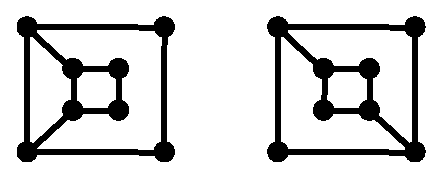
\includegraphics[width=.5\textwidth]{non_iso_graphs.eps}
    \label{fig:non-iso_graphs}
    \caption{Two non-isomorphic graphs}
\end{center}
\end{figure}

\begin{exercises}
\begin{enumerate}
    \item Let $v$ be a natural number.  The \textbf{wheel graph} on $v$ vertices, denoted $W_v$, is the graph obtained from $C_{v-1}$ by adding a new ``complete'' vertex, \textit{i.e.} a vertex that is adjacent to every other vertex.  Draw some examples of wheel graphs, then determine and prove the correctness of a formula for the number of edges in $W_v$.
    \item Let $G$ be a graph.  Determine and prove correctness of a formula for the number of edges in $\overline{G}$ given only $v(G)$ and $e(G)$.
    \item Determine all numbers $v$ such that $C_v \cong K_v$. Prove your claim.
    \item The degree sequence is what is called an \textbf{isomorphism invariant} meaning that if $G \cong H$, then the degree sequence of $G$ equals the degree sequence of $H$ (by Theorem \ref{thm:degree_seq_invt}).  State the contrapositive of this statement, and find a pair of graphs with the same number over vertices (at least 5), edges (at least 7), yet a different degree sequence.  What can you conclude about these graphs?  Find a pair of non-isomorphic graphs with at least 5 vertices, none of degree 2, for which their degree sequences do not prove their non-isomorphic status.  This shows that the degree sequence is not a \textit{complete} invariant.
    \item Prove that $C_v \cong \overline{C_v}$ if and only if $v = 5$.
    \item Prove that if $G \cong \overline{G}$, then $v$ or $v-1$ is divisible by 4.
    \item Prove that if $G_1 \cong G_2$ and $A_1 \subseteq G_1$ then there exists a subgraph $A_2 \subseteq G_2$ with $A_1 \cong A_2$.  Use this to reprove the non-isomorphism of Example \ref{ex:non-iso_graphs}.
    \item Classify all graphs with 3 vertices up to isomorphism.  That is, find a list of pairwise non-isomorphic graphs such that any graph with 3 vertices is isomorphic to exactly one of the graphs in your list.
    \item Prove that $G_1 \cong G_2$ if and only if $\overline{G_1} \cong \overline{G_2}$.
    \item A \textit{partition} of a set is a decomposition into non-intersecting sets.  That is, $\{1,2,3\} = \{1,2\} \cup \{3\}$ is a partition, but $\{1,2,3\} = \{1,2\} \cup \{2, 3\}$, which is a true statement, is not a partition.

    Let $G$ be a graph such that $V(G)$ can be partitioned into two sets $A$ and $B$ with the property that no edges of $G$ have both vertices in $A$ or both vertices in $B$.  Then $G$ is called a \textbf{bipartite graph}.

    One family of examples of bipartite graphs are the \textbf{complete bipartite graphs}, $K_{m,n}$: given natural numbers $m$ and $n$, the complete bipartite graph on $m$ and $n$ vertices is a bipartite graph with partition $A\cup B$, where $|A| = m$ and $|B| = n$, and all possible edges.  Draw some examples of complete bipartite graphs.

    Let $m$, $n$, $a$, and $b$ be natural numbers. Prove that $K_{m,n} \cong K_{a,b}$ if and only if $m = a$ and $n = b$.

    \item Create formulae (and prove their correctness) for the number of edges of each of the following families of graphs, based on the number of vertices ($v$):
    \begin{itemize}
        \item $K_v$
        \item $C_v$
        \item $\overline{C}_v$
        \item $W_v$ (wheel graph)
        \item $K_{m,n}$.
    \end{itemize}

    \item Prove that a graph with $v \geq 2$ has two vertices with the same degree.

\end{enumerate}
\end{exercises}


\newpage
\section{Planar Graphs} \label{sec:planar}

This is the section on planar graphs, still to be completed.

\begin{itemize}
    \item Definition of graph projection
    \item A Graph is planar if it (is isomorphic to?) a graph with a projection drawn in a plane with no edge-crossings (define)
    \item examples
    \item Jordan Curve Theorem: If $C$ is a continuous simple closed curve in a plane and two points $x$ and $y$ of $C$ are joined by a continuous simple arc $L$ such that $L \cap C = \{x, y\}$, then except for its endpoints $L$ is entirely contained in one of the two regions of $\R^2 \setminus C$.
    \item $K_{3,3}$ is nonplanar (not using Euler)
    \item $K_5$ is nonplanar
    \item Any subgraph of a planar graph is planar
    \item corollary any supergraph of a nonplanar graph is nonplanar
    \item If $G$ may be obtained from $H$ by replacing an edge $(x, y)$ of $H$ with another vertex $v$, and a pair of edges $(x, v), (v, y)$, then $G$ is said to be obtained from $H$ via an \textbf{edge expansion}.  If $G$ may be obtained from $H$ by a finite sequence of edge expansions, then $G$ is an \textbf{expansion} of $H$.
    \item (maybe?) If $G$ is obtained from $H$ by a sequence of expansions and passing to supergraphs, then $G$ is said to be an \textbf{expanded supergraph} of $H$ (my definition) (NOTE: this is equivalent to being a supergraph of an expansion.  Prove!)
    \item Every expanded supergraph of $K_{3,3}$ or $K_5$ is nonplanar.
    \item Kuratowski's Theorem: a graph is nonplanar if and only if it is an expanded supergraph of $K_{3,3}$ or $K_5$.
    \item exercise: examples of large graphs, is it planar?

    \item TODO: add exercises
\end{itemize}

% Should this be its own chapter?  Included in the current chapter?
\section{Euler's Formula}
\begin{itemize}
    \item A \textbf{walk}, or \textbf{path} is a sequence $v_1, v_2, \ldots, v_n$ of not-necessarily-distinct vertices in a graph $G$ such that $(v_i, v_{i+1})$ is an edge of $G$ for $1\leq i <n$.
    \item A graph is \textbf{connected} if every pair of vertices may be joined by a path.  Otherwise, it is disconneted
    \item Disclaimer: path connected vs connected?
    \item examples
    \item Given a planar graph diagram $D$, a \textbf{face} of $D$ is the set of all points in $\R^2 \setminus D$ that may be joined by a continuous arc in $\R^2 \setminus D$.  The number of faces of $D$ is denoted as
    \item prove if $G$ is a planar graph, then the number of faces of \textit{any} planar diagram of $G$ is the same.
    \item A graph is \textbf{polygonal} if it is planar, connected, and has the propery that every edge borders on two different faces
    % \item Induction?  Probably covered in the combinatorics section.
    \item If $G$ is polygonal then $v-e+f = 2$. (two students, longish)
    \item If $G$ is planar and connected, then $v-e+f = 2$.
    \item $K_5$ and $K_{3,3}$ are nonplanar, revisited.
    \item If $G$ is planar (and connected? not necessary) then $G$ has a vertex of degree $\leq 5$ (Q?)
    \item exercises from 4
    \item a graph is \textbf{regular} if all its vertices have the same degree, said ``regular of degree $d$''.
    \item examples
    \item a graph is \textbf{platonic} if it is polygonal, regular, and all its faces are bounded by the same number of edges
    \item (what if we remove the last condition?)
    \item examples
    \item Theorem: Apart from $K_1$ and the cyclic graphs, there are 5 platonic graphs.  Prove by breaking into $d$ cases Needs lemata:
    \begin{itemize}
        \item if $G$ is regular of degree $d$ then $e=dv/2$.
        \item If $G$ is platonic of degree $d$, and $n$ is the number of edges bounding each face, then $f = dv/n$.
    \end{itemize}
    \item exercises
\end{itemize}


\newpage
\bibliographystyle{amsalpha}
\bibliography{MasterBibliography}
\end{document}
